\section{CAG Register File Generator}

To resolve the problems connected with commercial tools for RFs the Computer Architecture Group (CAG) of the Heidelberg University is developing its own tool called Register File Generator (RFG). It is an open source project and publicly available at \emph{github.com/unihd-cag/odfi-rfg}.

\subsection{RFG Terminology}\label{section::rfg_term}

The RFG uses two interfaces to access the generated RF (fig.~\ref{fig::rfg_view}). On one side a bus, which enables access to the RF from outside the hardware and is called software view. Its signals are shared between the registers of the RF and a specific CSR is accessed via its address. Thereby different read or write commands targeting the RF can only be executed sequentially.\\
On the contrary the logic of the hardware is directly connected to each of its corresponding registers (except memory based registers as described in section~\ref{section::ramblocks}). Therefore the interface of the hardware view does not represent an uniform set of signals, but rather an aggregation of point-to-point connections, which depends on the registers of the RF.

\begin{figure}[h]
 \centering
 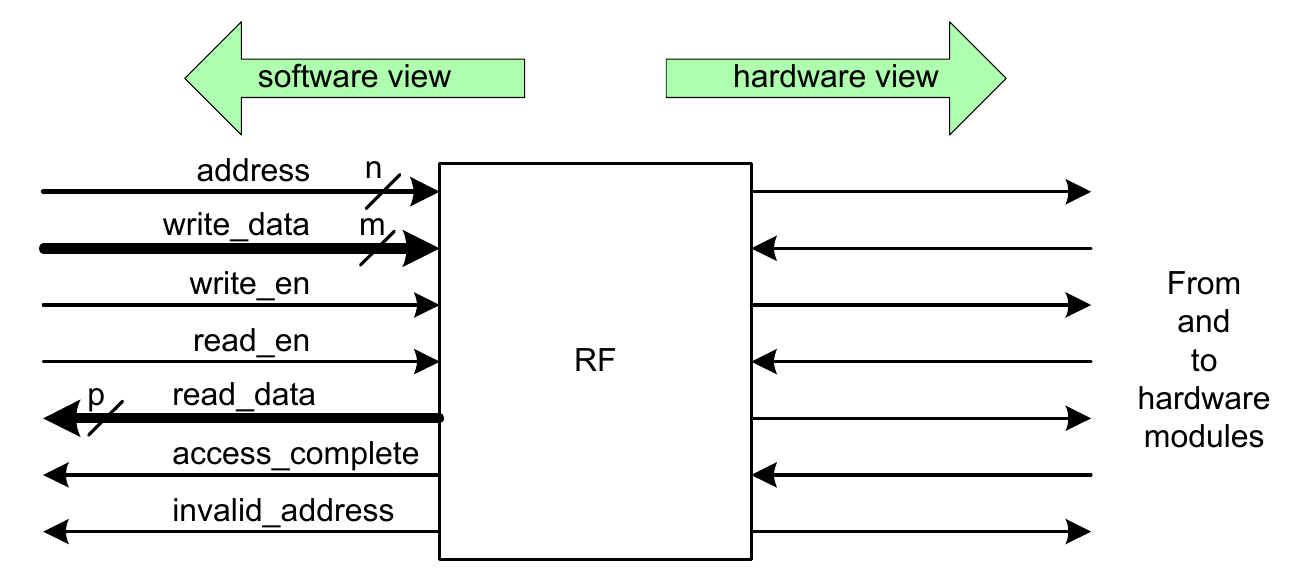
\includegraphics[width=252pt]{images/rf_view.png}
 \caption{RFG Terminology \cite{leber_diss}}
\label{fig::rfg_view}
\end{figure}
Following the timing diagrams of a read respectively write access on the software interface are shown.\\
When reading a register (fig.~\ref{fig::sw_read}), the \lstinline$address$ of the register has to be applied simultaneously with the assertion of the \lstinline$read_en$ signal. Thereby, \lstinline$read_en$ has to be active for a single clock cycle. Otherwise multiple reads could be detected instead of the desired single one. When the data of the register is available at \lstinline$read_data$, the RF asserts the \lstinline$access_complete$ signal for a single clock cycle. Thereby, the read data is only valid for this clock cycle. After that, the software bus is again available for the next read or write access.\\
\begin{figure}[h]
 \centering
 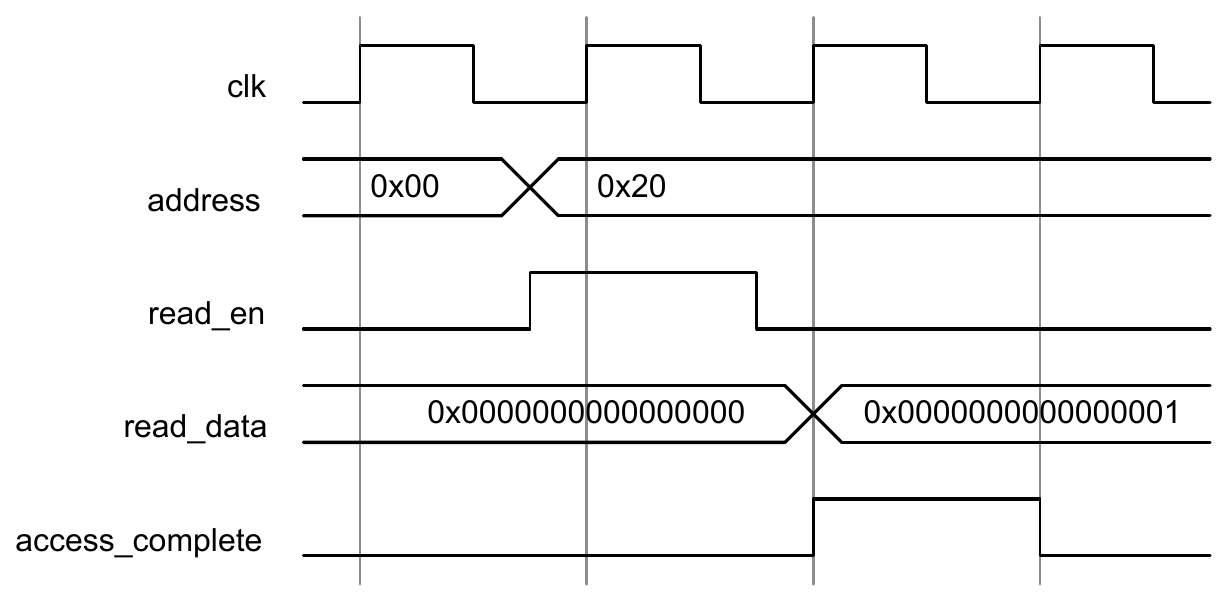
\includegraphics[width=252pt]{images/sw_read_timing.png}
 \caption{Timing Diagram of a SW Read Access \cite{leber_diss}}
\label{fig::sw_read}
\end{figure}
A write access (fig.~\ref{fig::sw_write}) is performed by applying the address of the destination register to the \lstinline$address$ signal and the data to \lstinline$write_data$. This has to be done simultaneously with the assertion of \lstinline$write_en$ for a single clock cycle. When the write access is complete, the RF asserts \lstinline$access_complete$ for a single clock cycle. After that, the software bus is again available for the next read or write access.
\begin{figure}[h]
 \centering
 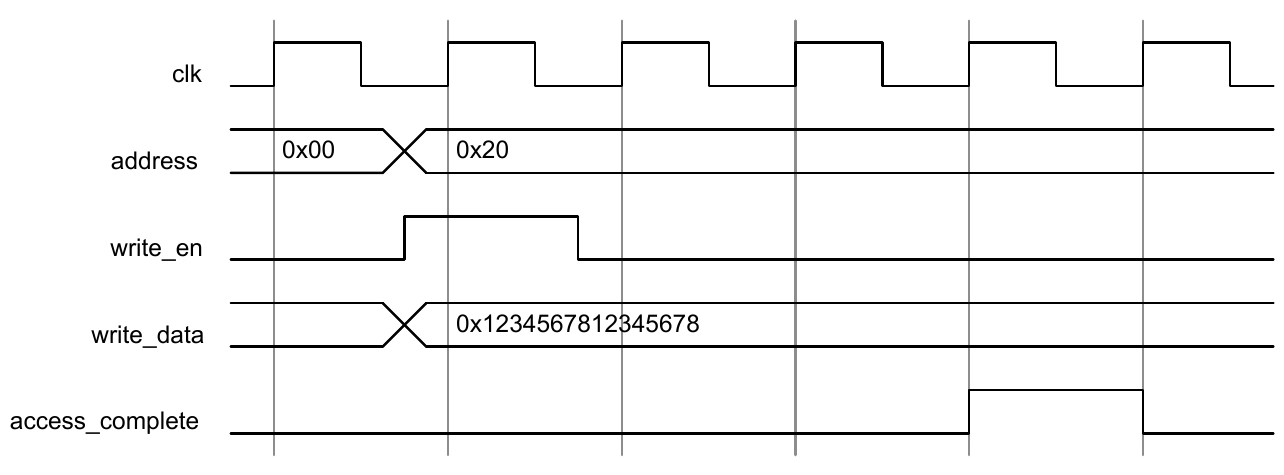
\includegraphics[width=252pt]{images/sw_write_timing.png}
 \caption{Timing Diagram of a SW Read Access \cite{leber_diss}}
\label{fig::sw_write}
\end{figure}

\subsection{RFG Components}
An example of a RF description for the RFG is given in listing~\ref{lst::example_rf}. Following is described, which components are available at the RFG to describe a RF and how they are used.

\lstset{language={}, numbers=none, escapechar=|}
\begin{lstlisting}[frame=single,
caption={Example RF description},
basicstyle=\small\ttfamily,
label={lst::example_rf}]
registerFile rf_top {

  register reg0 {
    field field0 {
      width 32
      software {
        rw
      }
      hardware {
        rw
        clear
      }
    }
    reserved 32
  }
	
  ramBlock ram0 {
    width 64
    depth 32
    software rw
    hardware rw
  }
	
  external rf_inner.rf example
}
\end{lstlisting}

\subsubsection{Register Files}
A RF is the top module containing all other components like registers and ramblocks. It is declared using \lstinline$registerFile$ followed by its name.
Furthermore hierarchical RFs are available, which split the RF in multiple sub-RFs. On the one hand this can resolve timing problems in large designs (see section~\ref{rf_generation}), on the other hand the RF obtains a clear structure and is therefore better to maintain than a non-hierarchical one.\\
A hierarchical RF is created by using the \lstinline$external$ statement followed by the filename of the included RF and the name of the RF. Each RF respectively sub-RF is declared in an individual file using the filename extension \lstinline$.rf$.
\subsubsection{Registers}
CSRs are declared inside of an RF using the \lstinline$register$ statement followed by an unique name in the scope of the enclosing RF. The width of the registers is declared globally and has the default value of 64 bit. Each register can contain multiple fields with variable width. Thereby, unused bits can be marked with the \lstinline$reserved$ statement. Furthermore read and write permissions can be assigned to each field for both software and hardware view.\\
In addition to the basic CSRs, more specialized registers can be created with this generator. This is achieved by assigning flags to the fields of the register in the RF description called attributes. For example, a counter can be added to the RF by using the corresponding attribute (see \cite{rfg_spec} for a list of available attributes).
\subsubsection{Ramblocks}\label{section::ramblocks}
The RFG also supports memory type registers in static random-access memories (SRAMs) called ramblocks. These are used when the same kind of register is required multiple times with consecutive addresses. It is important to mention, that in this case the hardware is not directly connected to the fields. Instead the logic can only use an SRAM interface to read or write an entire entry of the memory, which is similar to accessing a complete register. Additionally registers combined in a single ramblock can only be accessed sequentially due to the capabilities of the SRAM interface.\\
Analogous to the fields of registers, read and write permissions for software and hardware view can be specified for ramblocks. Additionally each ramblock can either be internal (default value) or external. Internal ones are instantiated within the RF, whereas an external ramblock only includes an SRAM interface inside of the RF and the developer has to connect it.
\subsection{Verification Model}
The RFG contains multiple generators. Each creating a different part of the RF. Among these are generators for hardware description, documentation as well as a verification model. Following, the verification model will be presented, as an example for such a generator.\\
When verifying a design, tests have to be created, which generate the stimulus signals for the device under test (DUT). This has to be done manually, because it depends on the logic connected to the RF and cannot be done in a general manner for different RFs. In case of the software interface of the RF this means creating sets of read and write accesses for the distinct registers. As mentioned in section~\ref{section::rfg_term}, CSRs are accessed via the software bus of the RF using the address of the register. However, the RF description is independent of these addresses. They are not determined until the register file generation is invoked. This has the advantage, that additional registers can be easily added to an existing RF without adjusting the descriptions of the other CSRs. Due to such extensions of the RF during the design process, the address mapping of the RF can change multiple times. This leads to the need of constantly adjusting the tests of the verification environment according to the changes in the address map of the RF.\\
This is contrary to the purpose of a register file generator to eliminate such time consuming and error prone tasks. Therefore it seems natural to create tests for the software interface, which are independent of addresses. This is achieved by using a model of the RF, which maps the name of a CSR to its corresponding address. Thereby, a register can be accessed without explicitly knowing its address inside of the RF.\\
In this way, the existing tests can be left unchanged, when CSRs are added to the RF. Just the verification model has to be generated again to include the new address mapping.\\
The model is available for two major verification frameworks, UVM-\textit{e} as well as UVM-SystemVerilog. It does not use absolute addresses for its components. Instead, each component has an address relative to its enclosing RF (fig.~\ref{fig::rel_address}). This uses the availability of hierarchical RFs in the RFG. The absolute address of a component is determined by the sum of its own relative address and all parent components until the top RF is reached. The address of an entry of a ramblock is composed of the address of the entry inside the ramblock and the address of the ramblock itself.\\ Additionally, an existing verification model can be used as sub-RF in other models without the need of generating it again to update the address mapping. That is the reason for using relative addresses inside of the verification models.
\begin{figure}[h]
 \centering
 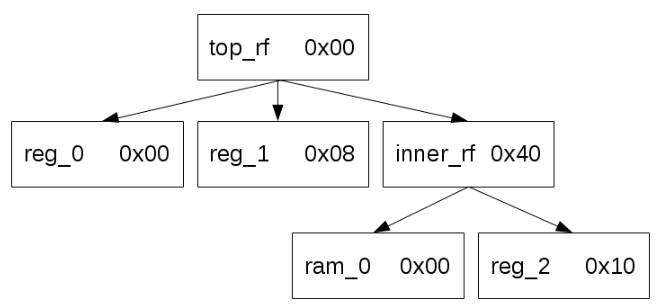
\includegraphics[width=252pt]{images/hierarchy_rf.png}
 \caption{Relative Addresses of the RF Verification Model}
\label{fig::rel_address}
\end{figure}
